\documentclass{standalone}
\usepackage{tikz}
\usetikzlibrary{decorations.pathmorphing}
\begin{document}
\tikzset{
    decorated/.style={
        postaction={decorate},
        decoration={
            snake,
            amplitude=1mm,
            segment length=6mm,
        }
    },
}
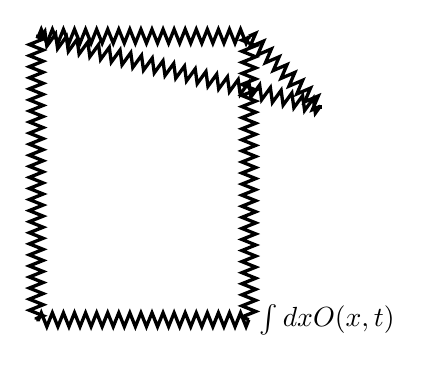
\begin{tikzpicture}[>=stealth,very thick,scale=.9]
    \draw[decoration={zigzag,segment length=4pt},decorate] (0,-2)--(0,2);
    \draw (1,1) node[rectangle,fill,inner sep=0pt,minimum size=0.5mm]{};
    \draw[decoration={zigzag,segment length=4pt},decorate] (-3,2)--(-3,-2);
    \draw[decoration={zigzag,segment length=4pt},decorate] (0,-2)--(-3,-2);
    \draw[decoration={zigzag,segment length=4pt},decorate] (0,2)--(-3,2);
    \draw[decoration={zigzag,segment length=4pt},decorate] (0,2)--(1,1);
    \draw[decoration={zigzag,segment length=4pt},decorate] (1,1)--(-3,2);
    \node[right] at (0,-2) {$\int dxO(x,t)$};
\end{tikzpicture}
\end{document}